\section{Pianificazione}
In questa sezione verrà riportata la pianificazione di progetto prevista dal gruppo Catch Em
All. La pianificazione è stata suddivisa nelle seguenti fasi:
\begin{itemize}
	\item Analisi;
	\item Sviluppo del Proof of Concept;
	\item Progettazione architetturale;
    \item Progettazione di dettaglio e Codifica;
	\item Validazione e Collaudo.
\end{itemize}

\subsection{Analisi}
Questa fase ha lo scopo di analizzare in dettaglio il capitolato scelto dal gruppo in modo da definire gli obiettivi funzionali, i tempi e i costi del progetto, e gli obiettivi di qualità.

\subsubsection{Periodo}
La fase di analisi si svolgerà dal 07/11/2022 fino al 08/01/2023.

\subsubsection{Precondizioni}
\begin{itemize}
	\item E’ stato formato il gruppo Catch Em All;
	\item E’ stato assegnato il capitolato d’appalto C1: “Captcha: umano o sovrumano?”.
\end{itemize}

\subsubsection{Postcondizioni}
Stesura e verifica dei seguenti documenti:
\begin{itemize}
	\item Norme di Progetto;
	\item Analisi dei Requisiti;
	\item Glossario;
    \item Piano di Progetto;
	\item Piano di Qualifica.
\end{itemize}

\subsubsection{Attività}
\begin{itemize}
	\item \textbf{Scelta degli strumenti}: Individuazione e studio di tutti gli strumenti utili nella stesura della documentazione e sviluppo del prodotto;
    \item \textbf{Norme di Progetto}: Stesura del documento contenente le linee guida a cui il gruppo si atterrà per tutte le altre attività di progetto;
    \item \textbf{Analisi dei Requisiti}: Attività finalizzata alla comprensione dei bisogni espressi nel capitolato d’appalto e ricavati dallo studio del dominio d’uso; i requisiti individuati verranno classificati nel documento Analisi dei Requisiti, il quale conterrà anche i casi d’uso corredati da diagrammi UML;
    \item \textbf{Glossario}: Al fine di evitare le ambiguità che si possono creare utilizzando il linguaggio naturale nella stesura dei documenti, le parole chiave utili alla comprensione del dominio d’uso verranno raccolte nel Glossario;
    \item \textbf{Piano di Progetto}: Stesura del documento che riporta la pianificazione di progetto prevista dal gruppo, la distribuzione delle ore di lavoro e il prospetto dei costi;
    \item \textbf{Piano di Qualifica}: Stesura del documento dove vengono definiti gli obiettivi di qualità per i processi e i prodotti di progetto, e con quali metodi e strumenti si svolgeranno le attività di verifica e validazione.
\end{itemize}

\subsubsection{Ruoli attivi}
Durante la fase di analisi saranno necessari i seguenti ruoli:
\begin{itemize}
	\item Responsabile;
    \item Amministratore;
    \item Analista;
    \item Verificatore.
\end{itemize}

\subsubsection{Suddivisione temporale}
La fase di analisi è stata suddivisa in tre periodi distinti, elencati ed analizzati di seguito.

\subsubsubsection{Primo periodo}
\begin{itemize}
    \item Dal 07/11/2022 al 27/11/2022.
\end{itemize}
Nel primo periodo il gruppo effettua un’analisi preliminare e avvia le attività di stesura delle bozze di alcuni documenti elencati al paragrafo 4.1.2 Postcondizioni - in particolare Norme di Progetto, Analisi dei Requisiti e Piano di Progetto - impostandone la struttura principale. Vengono inoltre scelti gli strumenti da utilizzare per la stesura di tali documenti e redatti i primi verbali in modo da tenere traccia delle riunioni interne e col proponente.

\subsubsubsection{Secondo periodo}
\begin{itemize}
    \item Dal 28/11/2022 al 25/12/2022.
\end{itemize}
Nel secondo periodo vengono redatti i documenti abbozzati nel primo periodo, partendo dalle Norme di Progetto e Analisi dei Requisiti. Viene anche iniziata la stesura del Piano di Qualifica e Glossario.
A ciascun membro del gruppo vengono affidati dei compiti specifici per ogni sprint. Iniziano anche le attività di verifica incrementale per i documenti in corso di stesura, in modo da monitorare costantemente gli avanzamenti.

\subsubsubsection{Terzo periodo}
\begin{itemize}
    \item Dal 26/12/2022 al 08/01/2023.
\end{itemize}
Nel terzo periodo il gruppo effettua le attività di verifica finale sui documenti prodotti nel secondo periodo per assicurarsi che i documenti siano coerenti fra loro, conformi alle linee guida stabilite nelle Norme di Progetto, e pronti per la revisione RTB.

\subsubsection{Diagramma di Gantt - Analisi}

\begin{figure}[H]
\centering
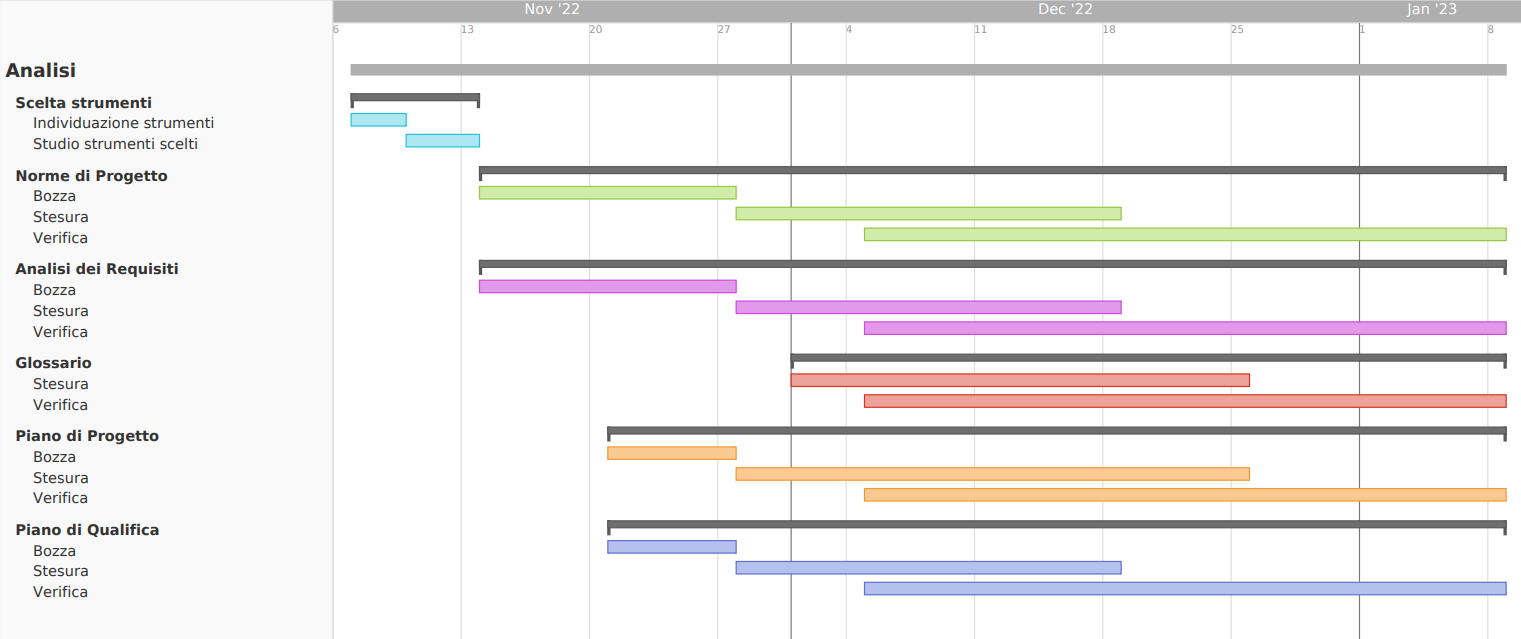
\includegraphics[width=\textwidth]{img/4_analisi.png}
\caption{Analisi}
\end{figure}

\subsection{Produzione del Proof of Concept}
Gli obiettivi di questa fase sono lo studio delle possibili soluzioni architetturali per il PoC e l’individuazione dell’architettura di base per l’implementazione del prodotto. Segue a ciò l’attività di codifica del PoC.\\
La fase di produzione del Proof of Concept terminerà con la prima revisione RTB.

\subsubsection{Periodo}
La fase di produzione del Proof of Concept si svolgerà dal 09/01/2023 fino al 30/01/2023.

\subsubsection{Precondizioni}
I seguenti documenti sono stati redatti e verificati:
\begin{itemize}
	\item Norme di Progetto;
	\item Analisi dei Requisiti;
	\item Glossario;
    \item Piano di Progetto;
	\item Piano di Qualifica.
\end{itemize}

\subsubsection{Postcondizioni}
\begin{itemize}
	\item Aggiornamento e miglioramento dei documenti in precedenza redatti durante la fase di Analisi;
	\item Sviluppo del PoC;
	\item Preparazione presentazione per la revisione RTB.
\end{itemize}

\subsubsection{Attività}
\begin{itemize}
	\item \textbf{Aggiornamento e miglioramento dei documenti}: Attività finalizzata a migliorare, se necessario, i documenti prodotti nella fase precedente aggiungendo nuovi elementi;
	\item \textbf{Individuazione requisiti per il PoC}: Attività di analisi finalizzata all’individuazione dei requisiti che il PoC andrà a soddisfare;
    \item \textbf{Progettazione Technology Baseline}: Individuazione dell’architettura di base per l’implementazione del prodotto;
        \subitem \textbf{Approfondimento sulle tecnologie scelte}: I membri del gruppo si dedicano allo studio individuale delle tecnologie selezionate; al termine di questa attività tutti avranno acquisito le competenze necessarie per poter lavorare a rotazione sulla produzione del PoC;
    \item \textbf{Sviluppo della Technology Baseline}: Attività di codifica e verifica del PoC;
    \item \textbf{Preparazione della presentazione per la revisione RTB}: : Il gruppo si dedica alla preparazione dell’esposizione degli obiettivi raggiunti.
\end{itemize}

\subsubsection{Ruoli attivi}
Durante la fase di produzione del Proof of Concept lisi saranno necessari i seguenti ruoli:
\begin{itemize}
	\item Responsabile;
    \item Amministratore;
    \item Analista;
    \item Progettista;
    \item Programmatore;
    \item Verificatore;
\end{itemize}

\subsubsection{Suddivisione temporale}
La fase di produzione del Proof of Concept è stata suddivisa in due periodi, analizzati di seguito. La milestone individuata è rappresentata dalla revisione RTB.

\subsubsubsection{Primo periodo}
\begin{itemize}
    \item dal 09/01/2023 al 15/01/2023
\end{itemize}
Nel primo periodo vengono individuati i requisiti in base ai quali produrre il PoC e selezionata l’architettura di base per la sua implementazione. Ciascun membro del gruppo si impegna ad approfondire autonomamente le tecnologie scelte e colmare eventuali lacune nelle conoscenze di strumenti, librerie e così via. Viene anche iniziato l'aggiornamento, se necessario, della documentazione prodotta nella fase precedente.

\subsubsubsection{Secondo periodo}
\begin{itemize}
    \item Dal 16/01/2023 al 30/01/2023
\end{itemize}
Nel secondo periodo viene effettuata la codifica e verifica del PoC, al termine delle quali il gruppo si dedica alla preparazione della presentazione per la revisione RTB.

\subsubsection{Diagramma di Gantt - Produzione del Proof of Concept}

\begin{figure}[H]
\centering
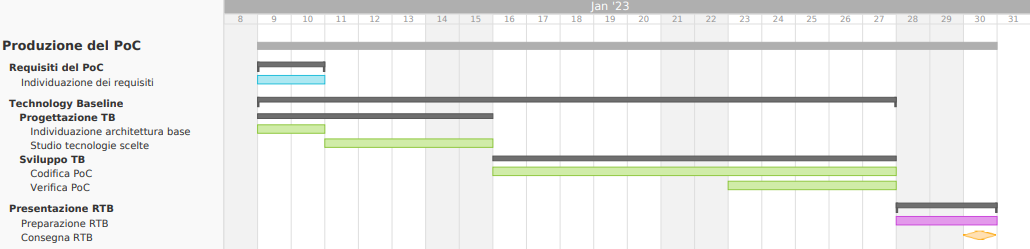
\includegraphics[width=\textwidth]{img/4_produzione.png}
\caption{Produzione del Proof of Concept}
\end{figure}

\subsection{Progettazione architetturale}
Lo scopo di questa fase è il raffinamento della progettazione architetturale ad alto livello avviata nella fase descritta al paragrafo 4.2 Produzione del Proof of Concept, ovvero “come” saranno soddisfatti i requisiti precedentemente individuati.
Le scelte che il gruppo effettua in questa fase riguarderanno la struttura complessiva del sistema e ne influenzeranno varie caratteristiche qualitative come per esempio l’efficienza, l’estensibilità e la manutenibilità.

\subsubsection{Periodo}
La fase di progettazione architetturale si svolgerà dal 31/01/2023 fino al 19/02/2023.

\subsubsection{Precondizioni}
\begin{itemize}
    \item E’ stato prodotto il PoC;
    \item Superamento della prima revisione (RTB).
\end{itemize}

\subsubsection{Postcondizioni}
\begin{itemize}
    \item Conclusione della progettazione architetturale ad alto livello.
\end{itemize}

\subsubsection{Attività}
\begin{itemize}
    \item \textbf{Incremento e verifica dei documenti}: A seconda delle necessità, il gruppo si occupa di aggiornare la documentazione prodotta in precedenza;
    \item \textbf{Progettazione architetturale}: Raffinamento della progettazione architetturale ad alto livello;
        \subitem \textbf{Approfondimento sulle tecnologie scelte}: I membri del gruppo si dedicano allo studio individuale delle tecnologie selezionate; al termine di questa attività tutti avranno acquisito le competenze necessarie per poter lavorare a rotazione sulla futura realizzazione del prodotto.
\end{itemize}

\subsubsection{Ruoli attivi}
Durante la fase di progettazione architetturale saranno necessari i seguenti ruoli:
\begin{itemize}
	\item Responsabile;
    \item Amministratore;
    \item Progettista;
    \item Verificatore.
\end{itemize}

\subsubsection{Suddivisione temporale}
La fase di progettazione architetturale è stata suddivisa in due periodi, analizzati di seguito.

\subsubsubsection{Primo periodo}
\begin{itemize}
	\item dal 31/01/2023 al 05/02/2023.
\end{itemize}
Nel primo periodo vengono aggiornati e migliorati i documenti redatti in precedenza in base al feedback ricevuto durante la revisione RTB.

\subsubsubsection{Secondo periodo}
\begin{itemize}
	\item dal 06/02/2023 al 19/02/2023.
\end{itemize}
Nel secondo periodo viene conclusa la progettazione architetturale; le soluzioni scelte punteranno alla correttezza per costruzione. Ciascun membro del gruppo si impegna ad approfondire autonomamente le tecnologie scelte nel secondo periodo e colmare eventuali lacune nelle conoscenze di strumenti, librerie e così via.

\subsubsection{Diagramma di Gantt - Progettazione architetturale}

\begin{figure}[H]
\centering
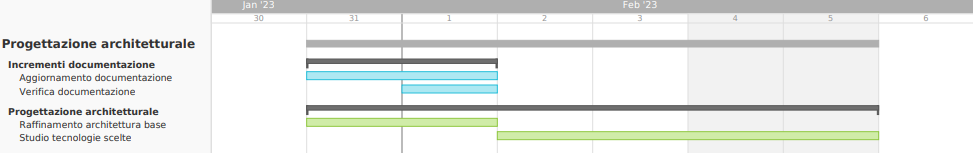
\includegraphics[width=\textwidth]{img/4_progettazione.png}
\caption{Progettazione architetturale}
\end{figure}

\subsection{Progettazione di dettaglio e Codifica}
Questa fase ha lo scopo di avviare le attività riguardanti la progettazione di dettaglio del sistema e la codifica del prodotto.
In particolare, la codifica si svolgerà in base alle norme di codifica stabilite nelle Norme di Progetto e avrà tra gli obiettivi anche l’assicurarsi di scrivere codice facilmente verificabile per facilitare il lavoro della fase successiva. Questo in quanto l'efficacia dei metodi di verifica è strettamente legata alla qualità di strutturazione del codice. In questo modo non sarà necessario dipendere solo dalla verifica retrospettiva, il cui costo cresce con l'avanzare della fase di codifica.

\subsubsection{Periodo}
La fase di progettazione di dettaglio e Codifica si svolgerà dal 20/02/2023 fino al 02/04/2023.

\subsubsection{Precondizioni}
\begin{itemize}
    \item E’ stata conclusa la progettazione architetturale ad alto livello.
\end{itemize}

\subsubsection{Postcondizioni}
\begin{itemize}
    \item Conclusione della progettazione di dettaglio;
    \item Conclusione di codifica e verifica.
\end{itemize}

\subsubsection{Attività}
\begin{itemize}
    \item \textbf{Incremento e verifica dei documenti}: A seconda delle necessità, il gruppo si occupa di aggiornare la documentazione prodotta in precedenza;
    \item \textbf{Product baseline}: Vengono studiati in dettaglio i design pattern da utilizzare e prodotti relativi diagrammi;
        \subitem \textbf{Definizione delle unità software che comporranno il prodotto}: Il prodotto viene suddiviso in unità, ciascuna delle quali potrà essere realizzata da un singolo programmatore;
    \item \textbf{Codifica}: Utilizzando il PoC prodotto in precedenza come base, viene prodotto il restante codice; la codifica avverrà utilizzando un approccio incrementale, per cui ogni incremento sarà costituito dalla codifica di un determinato caso d’uso e produrrà valore aggiunto;
        \subitem \textbf{Verifica}: Il codice prodotto viene continuamente verificato, tramite tecniche di analisi statica e dinamica - quest’attività prepara il successo della fase di validazione;
    \item \textbf{Stesura dell’allegato tecnico}: Viene prodotto il documento che descrive le caratteristiche architetturali del prodotto;
    \item \textbf{Stesura del manuale per la manutenzione del prodotto}: Viene prodotto il manuale per la manutenzione e le estensioni future del prodotto;
    \item \textbf{Stesura del manuale utente}: Viene prodotto il manuale contenente le istruzioni di utilizzo del prodotto;
    \item \textbf{Preparazione della presentazione per la revisione PB}: Il gruppo si dedica alla preparazione dell’esposizione degli obiettivi raggiunti.
\end{itemize}

\subsubsection{Ruoli attivi}
Durante la fase di progettazione di dettaglio e Codifica saranno necessari i seguenti ruoli:
\begin{itemize}
	\item Responsabile;
    \item Amministratore;
    \item Progettista;
    \item Programmatore;
    \item Verificatore.
\end{itemize}

\subsubsection{Suddivisione temporale}
La fase di progettazione di dettaglio e Codifica è stata suddivisa in tre periodi distinti, analizzati di seguito. La milestone individuata è rappresentata dalla revisione PB.

\subsubsubsection{Primo periodo}
\begin{itemize}
    \item dal 20/02/2023 al 26/02/2023
\end{itemize}
Nel primo periodo viene conclusa la progettazione di dettaglio e iniziata la stesura dell’Allegato tecnico: a questo punto ogni attività di codifica può essere avviata in base alle scelte architetturali fatte dal gruppo.

\subsubsubsection{Secondo periodo}\begin{itemize}
    \item dal 27/02/2023 al 26/03/2023
\end{itemize}
Nel secondo periodo il gruppo si dedica alle attività di codifica e verifica. Ad ogni sprint review vengono analizzati i risultati raggiunti e studiato un piano di azione per lo sprint successivo, in modo da mantenere un’elevata capacità di rispondere alle eventuali problematiche riscontrate. Al termine di questo periodo il MVP è pronto per la revisione PB.

\subsubsubsection{Terzo periodo}
\begin{itemize}
    \item dal 27/03/2023 al 02/04/2023
\end{itemize}
Nel terzo periodo vengono redatti i manuali per la manutenzione e l’utilizzo del prodotto, e viene preparata la presentazione per la revisione PB.

\subsubsection{Diagramma di Gantt - Progettazione di dettaglio e Codifica}

\begin{figure}[H]
\centering
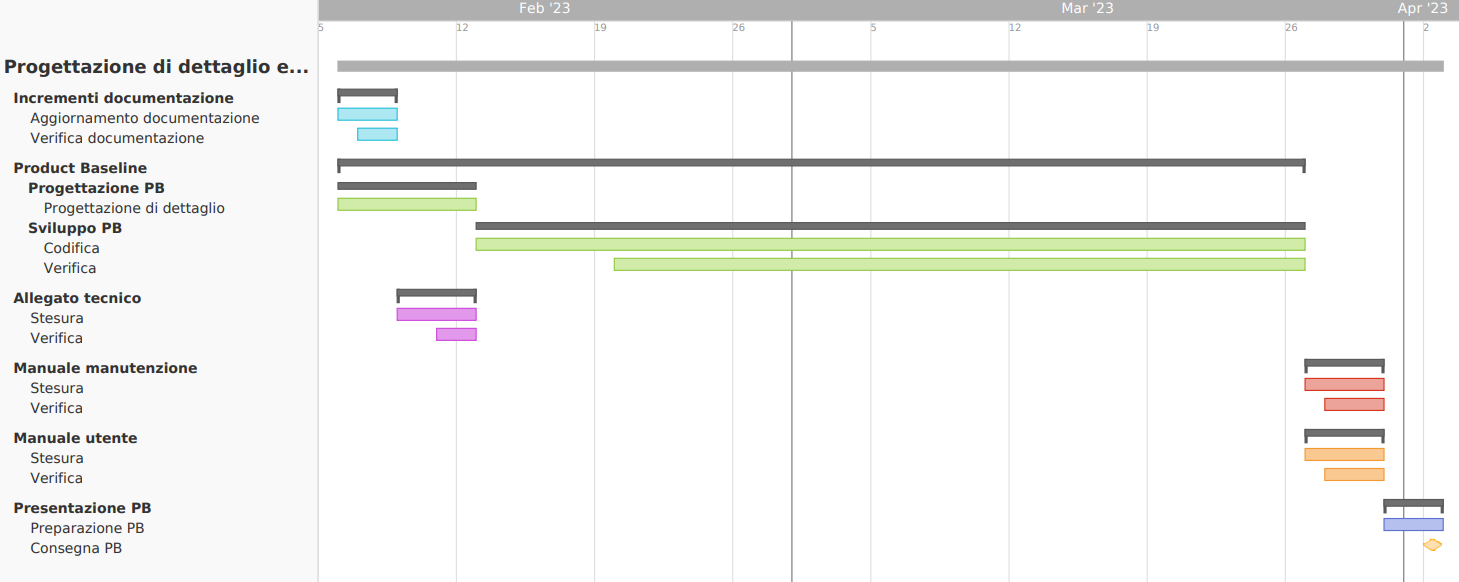
\includegraphics[width=\textwidth]{img/4_codifica.png}
\caption{Progettazione di dettaglio e Codifica}
\end{figure}

\subsection{Validazione e Collaudo}
In questa fase vengono effettuati i controlli necessari per garantire che il prodotto soddisfi le attese degli stakeholder: il progetto si conclude con una verifica del comportamento del sistema completo rispetto ai requisiti stabiliti in precedenza, in presenza del committente.

\subsubsection{Periodo}
La fase di Validazione e Collaudo si svolgerà dal 03/04/2023 fino al 30/04/2023.

\subsubsection{Precondizioni}
\begin{itemize}
    \item E’ stata conclusa la progettazione di dettaglio
    \item Sono state concluse la codifica e la verifica
\end{itemize}

\subsubsection{Postcondizioni}
\begin{itemize}
    \item Produzione dei test necessari
    \item Esecuzione e superamento di tutti i test
\end{itemize}

\subsubsection{Attività}
\begin{itemize}
    \item \textbf{Incremento e verifica dei documenti}: a seconda delle necessità, il gruppo si occupa di aggiornare la documentazione prodotta in precedenza
    \item \textbf{Validazione e Collaudo}: viene verificato che il prodotto finale soddisfi i requisiti stabiliti tenendo in considerazione anche gli obiettivi di qualità definiti nel Piano di Qualifica
    \item \textbf{Preparazione della presentazione per la revisione CA}: il gruppo si dedica alla preparazione dell’esposizione degli obiettivi raggiunti
\end{itemize}

\subsubsection{Ruoli attivi}
Durante la fase di Validazione e Collaudo saranno necessari i seguenti ruoli:
\begin{itemize}
	\item Responsabile
    \item Amministratore
    \item Programmatore
    \item Verificatore
\end{itemize}

\subsubsection{Suddivisione temporale}
La fase di Validazione e Collaudo è stata suddivisa in due periodi distinti, analizzati di seguito. La milestone individuata è rappresentata dalla revisione CA.

\subsubsubsection{Primo periodo}
\begin{itemize}
    \item dal 03/04/2023 fino al 24/04/2023
\end{itemize}
Nel primo periodo vengono effettuati tutti i test necessari; è possibile che in questo periodo sia necessario un incremento del codice in base ai risultati dei test.

\subsubsubsection{Secondo periodo}
\begin{itemize}
    \item dal 25/04/2023 fino al 30/04/2023
\end{itemize}
Nel secondo periodo il gruppo si dedica alla preparazione della presentazione per la revisione CA.

\subsubsection{Diagramma di Gantt - Validazione e Collaudo}

\begin{figure}[H]
\centering
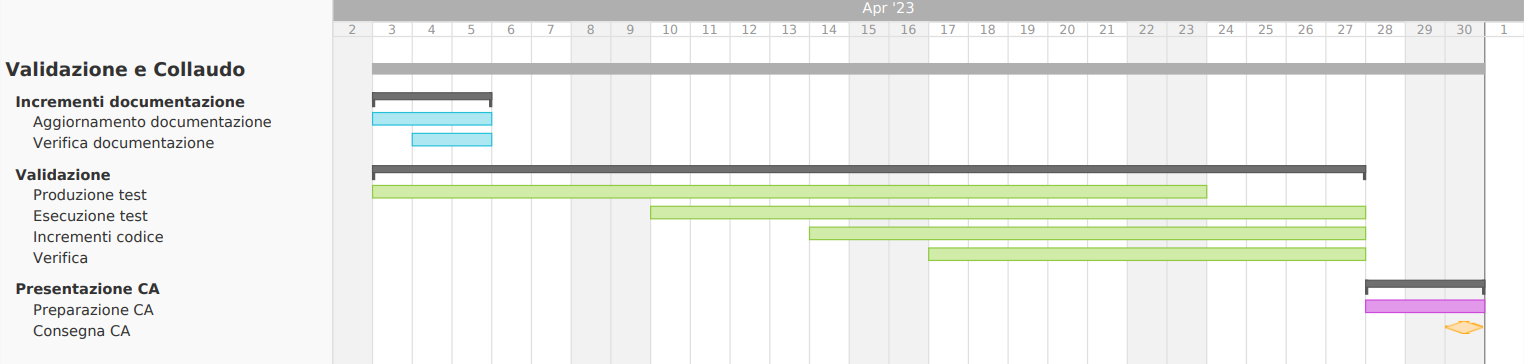
\includegraphics[width=\textwidth]{img/4_collaudo.png}
\caption{Validazione e Collaudo}
\end{figure}

